\documentclass[11pt,a4paper,titlepage]{article}
\usepackage[utf8]{inputenc}
\usepackage{amsmath}
\usepackage{amsfonts}
\usepackage{braket}
\usepackage{csvsimple}
\usepackage{amssymb}
\usepackage[ruled,vlined]{algorithm2e}
\usepackage{nameref}
\usepackage{subcaption}
\usepackage{hyperref}
\hypersetup{
    colorlinks=true,
    linkcolor=black,
    filecolor=black,
    urlcolor=cyan,
    citecolor=black,
}
\usepackage{tikz}
\usetikzlibrary{calc,patterns,angles,quotes,shapes.geometric, arrows}

\def\layersep{2.5cm}
\def\layersepSmall{1.2cm}

\tikzstyle{train} = [rectangle, rounded corners, minimum width=2.2cm, minimum height=1cm,text centered, draw=black, fill=red!30]
\tikzstyle{test} = [rectangle, rounded corners, minimum width=2.2cm, minimum height=1cm,text centered, draw=black, fill=green!30]
\tikzstyle{data} = [rectangle, rounded corners, minimum width=11.8cm, minimum height=1cm,text centered, draw=black, fill=gray!30]
\tikzstyle{MSE} = [rectangle, rounded corners, minimum width=1.4cm, minimum height=1cm,text centered, draw=black, fill=orange!30]
\tikzstyle{arrow} = [thick,->,>=stealth]

\usepackage{float}
%\usepackage{mathtools}
\usepackage{bm}
\usepackage[margin=1in]{geometry}

\title{Application of restricted Boltzmann machines to trapped interacting electrons}
\author{Adrian Martinsen Kleven}
\date{Autumn 2020}
\usepackage{hyperref}

\usepackage{natbib}
\usepackage{graphicx}
\graphicspath{{../Results/Report_Results/}} %Setting the graphicspath

\begin{document}

\maketitle
\tableofcontents
\listoffigures
\listoftables
\clearpage
\section{Abstract}
In this paper we examine systems of one and two trapped electrons in two dimensions using a restricted Boltzmann machine to represent the trial wave function. The ground state is approximated using variational Monte- Carlo methods and compared to analytical expressions for both the interacting and the non- interacting case provided by M. Taut. \cite{PhysRevA.48.3561}. We examine the spatial distribution of electrons for the two- dimensional systems and the convergence rates for stochastic gradient descent (SGD) and adaptive momentum gradient descent (ADAM). ADAM was shown to have far greater convergence rates and so was the optimizer of choice for numerical experiments. The convergence rates and errors for importance sampling and brute force sampling were compared for the same number of steps, and importance sampling, being far superior was used for every simulation. The local energy expectation values for single- electron systems were found to be in agreement with analytical results with standard deviations of order $\mathcal{O}(10^{-6}a.u.)$. The energy for two electrons in one dimension was calculated to be $0.97796656$ with a standard deviation of the order $\mathcal{O}(10^{-6}a.u.)$. A large discrepancy from the analytic value of $1.0$. Finally the energy for two interacting electrons was calculated to be $3.04450717a.u.$ with a standard deviation of $0.01146434a.u.$, slightly above the analytic value of $3.0a.u.$.

\section{Introduction}
The mathematical complexity of quantum mechanical many- body systems has brought on the necessity for numerical solutions. The quantum wave function has been successfully modelled using a restricted Boltzmann machine (RBM) in many- body lattice spin- systems \cite{Carleo602}. The purpose of this paper is to examine its applicability in estimating the upper bound for the ground state energy of interacting two- electron systems confined in a harmonic oscillator potential. To do this we perform numerical experiments of systems with known solutions and make an estimation of its accuracy.\\First we cover the bare minimum of theory for transforming the RBM joint probability distribution to something representing a wave function. We then cover the relevant expressions for computations in the model and the analytical values for the ground state energies. Because the exclusion principle is not taken into account, we only examine systems for at most two electrons.\\ We then cover the specifics for this particular implementation including the choice of sampler and optimization scheme. Ending with the results of the numerical experiments and a discussion of the results, the numerical stability, and the potential of the program.\\\\All energies are given in atomic units (a.u.) and length scales in fractions of the Bohr radius ($2\cdot a_0$).\\The program was implemented using c++ with post analysis, blocking, plotting being done via Python. All relevant files, including selected runs for testing can be found at \href{https://github.com/adrian2208/QM_RBM/tree/main/QM_RBM}{Github}.

\section{Theory}
We can approximate the upper bound for the ground state of a quantum mechanical system by using the variational principle. We propose a trial wave function with some variational parameters, then optimize the energy- expectation value with respect to those parameters. The Expectation value for the energy is given by 
\begin{equation}
\langle E\rangle=\frac{\langle\psi|H| \psi\rangle}{\langle\psi \mid \psi\rangle}.
\end{equation}
The probability distribution for the locations of the electrons are estimated using the Metropolis and Metropolis- Hastings algorithms. A discussion of these can be found here \cite{Project1}.
\subsection{The wave function}
The quantum mechanical wave function will be represented by a RBM. 
The joint probability distribution for a RBM is defined by the Boltzmann distribution
\begin{equation}\label{eq:F_rbm}
F_{r b m}(\mathbf{X}, \mathbf{H})=\frac{1}{Z} e^{-\frac{1}{T_{0}} E(\mathbf{X}, \mathbf{H})}
\end{equation}
where $Z$ is the partition function
\begin{equation}\label{eq:partition_function}
Z=\iint \frac{1}{Z} e^{-\frac{1}{T_{0}} E(\mathbf{x}, \mathbf{h})} d \mathbf{x} d \mathbf{h}.
\end{equation}
We set $T_0 = 1$ for simplicity. Here, $E$ is the configuration energy of the network. The configuration energy expression is unique to different problems. The one of interest to us is the Gaussian- Binary RBM whose joint probability distribution is given by equations \eqref{eq:F_rbm}, \eqref{eq:partition_function} and 
\begin{equation}
E(\mathbf{X}, \mathbf{H})=\frac{\|\mathbf{X}-\mathbf{a}\|^{2}}{2 \sigma^{2}}-\mathbf{b}^{T} \mathbf{H}-\frac{\mathbf{X}^{T} \mathbf{W H}}{\sigma^{2}}
\end{equation}
where $\mathbf{X}$ are the visible nodes corresponding to the coordinates of each particle, $\mathbf{H}$ are the hidden nodes. $\mathbf{a}$ and $\mathbf{b}$ are the visible and hidden biases respectively. $\mathbf{W}$ is the matrix of weights connecting nodes between layers. To elucidate the connection between the joint probability distribution and the wave function, the hidden nodes are summed over, giving a distribution solely dependent on $\mathbf{X}$.

\begin{equation}\label{eq:wavefunction}
\begin{aligned}
\Psi(\mathbf{X}) &=\frac{1}{Z} \sum_{\mathbf{h}} e^{-E(\mathbf{X}, \mathbf{h})}\\
&=\frac{1}{Z} \sum_{\left\{h_{j}\right\}} e^{-\sum_{i}^{M} \frac{\left(X_{i}-a_{i}\right)^{2}}{2 \sigma^{2}}+\sum_{j}^{N} b_{j} h_{j}+\sum_{i, j}^{M, N} \frac{x_{i} w_{i j h_{j}}}{\sigma^{2}}} \\
&=\frac{1}{Z} e^{-\sum_{i}^{M} \frac{\left(X_{i}-a_{i}\right)^{2}}{2 \sigma^{2}}} \prod_{j}^{N}\left(1+e^{b_{j}+\sum_{i}^{M} \frac{X_{i} w_{i j}}{\sigma^{2}}}\right)
\end{aligned}
\end{equation}
\subsection{The Hamiltonian}
The Hamiltonian of the system is given by a standard harmonic oscillator Hamiltonian with an included, idealized interaction term
\begin{equation}\label{eq:hamiltonian}
\hat{H}=\sum_{i=1}^{N}\left(-\frac{1}{2} \nabla_{i}^{2}+\frac{1}{2} \omega^{2} r_{i}^{2}\right)+\sum_{i<j} \frac{1}{r_{i j}}
\end{equation}
using natural units $\left(\hbar=c=e=m_{e}=1\right)$.
\subsection{The Local energy }
The local energy
\begin{equation}
E_{L}=\frac{1}{\Psi} \hat{\mathbf{H}} \Psi
\end{equation}
can be determined analytically (see \nameref{app_A}), giving the expression \eqref{eq:local_energy_derived}. The local energy has to be minimized with respect to the network parameters. The gradient for the expectation value of the local energy is given by equation \eqref{eq:lE_gradient} (see \nameref{app_B}).
\subsection{Analytic energies}\label{section: Analytic_energies}
The wave function for one electron in a harmonic oscillator potential in two dimensions is given by
\begin{equation}
\phi_{n_{x}, n_{y}}(x, y)=A H_{n_{x}}(\sqrt{\omega} x) H_{n_{y}}(\sqrt{\omega} y) \exp \left(-\omega\left(x^{2}+y^{2}\right) / 2\right)
\end{equation}
where $A$ is the normalization and $H_{n_{x}}$ are the Hermite polynomials corresponding to the principal quantum number $n_{x}$. In its ground state, the unperturbed wave function has a local energy of $\omega$. 
\subsubsection{Non- interacting}
The two- electron wave function is given by
\begin{equation}
\Phi\left(\boldsymbol{r}_{1}, \boldsymbol{r}_{2}\right)=\frac{C}{\sqrt{2}} \phi_{0, 0}(\boldsymbol{r}_{1})\phi_{0, 0}(\boldsymbol{r}_{2})\left\{ \xi_+(\boldsymbol{r}_{1})\xi_-(\boldsymbol{r}_{2})-\xi_+(\boldsymbol{r}_{2})\xi_-(\boldsymbol{r}_{1})\right\}
\end{equation}
where we have ensured anti- symmetry under interchange of electrons by taking the product of the symmetric spatial part and the anti- symmetric spin part. Because the Hamiltonian doesn't couple to the electron spins, the spin- expression will vanish in the local energy calculation. 
\begin{equation}
\frac{1}{\Phi\left(\boldsymbol{r}_{1}, \boldsymbol{r}_{2}\right)} \hat{\mathbf{H}}_0 \Phi\left(\boldsymbol{r}_{1}, \boldsymbol{r}_{2}\right) =\frac{1}{\phi_{0, 0}(\boldsymbol{r}_{1})\phi_{0, 0}(\boldsymbol{r}_{2}) } \left( \phi_{0, 0}(\boldsymbol{r}_{1})\hat{\mathbf{H}}_0\phi_{0, 0}(\boldsymbol{r}_{2}) + \phi_{0, 0}(\boldsymbol{r}_{2})\hat{\mathbf{H}}_0\phi_{0, 0}(\boldsymbol{r}_{1}) \right)
\end{equation}
\begin{equation}
E^0_L = 2\omega
\end{equation}

\subsubsection{Interacting}
The case for two interacting electrons in two dimensions has been provided by Taut \cite{PhysRevA.48.3561} and is given by 3 $a.u$ for the Hamiltonian \eqref{eq:hamiltonian}.
\section{Implementation}
\subsection{The Wave function}
The wave function \eqref{eq:wavefunction} is partly separable, meaning we can avoid a few calculations by factoring out the parts of the wave function that don't change when the position of one particle is changed, meaning the evaluation in \eqref{eq:T_prob} and \eqref{eq:A_prob} becomes somewhat faster.\\\\The value of $\sigma$ in the wave function is set to $1.0$ for all simulations.
\subsection{Optimization}
The optimization of the network parameters was done using gradient descent methods with the local energy as the cost function. The learning rate is denoted by $\eta$ and the parameters by $\alpha_{i}=a_{1}, \ldots, a_{M}, b_{1}, \ldots, b_{N}, w_{11}, \ldots, w_{M N}$.
\subsubsection{Cost function gradient}
To calculate the Cost function Gradient in equation\eqref{eq:lE_gradient}, the program needs to sample three different quantities to obtain their expectation values.
These are
\begin{equation}
\left\langle E_{L} \frac{1}{\Psi} \frac{\partial \Psi}{\partial \alpha_{i}}\right\rangle, \hspace{2mm}\left\langle E_{L}\right\rangle\textit{ and }\left\langle\frac{1}{\Psi} \frac{\partial \Psi}{\partial \alpha_{i}}\right\rangle.
\end{equation}
The relevant values can be found in \nameref{app_A} and \nameref{app_B}. 
\subsubsection{Stochastic Gradient Descent (SGD)}
SGD uses a fixed learning rate and the cost function gradient to update the current parameters according to 
$$
\alpha_i^{(t+1)} \leftarrow \alpha_i^{(t)}-\eta G^{(t)}.
$$
\subsubsection{Adaptive Momentum estimation (ADAM)}
ADAM is a method of optimization that utilizes a running average of previous gradients to inform the current learning step. the parameters  $\alpha_i^{(t+1)}$ at optimization step $t+1$ is updated according to
$$
\begin{array}{l}
m_{\alpha}^{(t+1)} \leftarrow \beta_{1} m_{\alpha}^{(t)}+\left(1-\beta_{1}\right) G^{(t)} \\
v_{\alpha}^{(t+1)} \leftarrow \beta_{2} v_{\alpha}^{(t)}+\left(1-\beta_{2}\right)\left(G^{(t)}\right)^{2} \\
\hat{m}_{\alpha}=\frac{m_{\alpha}^{(t+1)}}{1-\beta_{1}^{t+1}} \\
\hat{v}_{\alpha}=\frac{v_{\alpha}^{(t+1)}}{1-\beta_{2}^{t+1}} \\
\alpha_i^{(t+1)} \leftarrow \alpha_i^{(t)}-\eta \frac{\hat{m}_{\alpha}}{\sqrt{\hat{v}_{\alpha}}+\epsilon}
\end{array}
$$
with the values $\beta_{1} = 0.9$, $\beta_{2} = 0.999$ and $\epsilon = 10^{-8}$ chosen for this implementation. ADAM incurs a marginally greater overhead than SGD, so any improvement in convergence will be much more use than the cumulative overhead from just a few hundred cycles.
\subsection{The Metropolis Algorithm}
The Metropolis algorithm works by choosing one particle at random, adjusting its position then calculating the new value of the wave function that arises. The probability of accepting that move is then calculated from equation \eqref{eq:T_prob} where we assume that $ T\left(x\rightarrow x^{\prime}\right)= T\left(x^{\prime}\rightarrow x\right)$
\begin{equation}
A\left(x\rightarrow x^{\prime}\right)=\min \left(1, \frac{|\Psi\left(x^{\prime}\right)|^2}{|\Psi\left(x\right)|^2} \frac{T\left(x\rightarrow x^{\prime}\right)}{T\left(x^{\prime}\rightarrow x\right)}\right).\label{eq:T_prob}
\end{equation}
In this way, the Metropolis algorithm samples from a probability distribution using a biased random walker\cite{Project1}.
\subsubsection{Metropolis- Hastings}
The Metropolis- Hastings algorithm uses the Greens function solution to the Fokker- Planck equation \eqref{eq:FPEQ} as the transition probability which gives the acceptance probability
\begin{equation}
A\left(x\rightarrow x^{\prime}\right)=\min \left(1, \frac{|\Psi\left(x^{\prime}\right)|^2}{|\Psi\left(x\right)|^2} \frac{G\left(x,x^{\prime},\delta t\right)}{G\left(x^{\prime},x,\delta t\right)}\right)\label{eq:A_prob}
\end{equation}
\begin{equation}
\frac{\partial P(x, t)}{\partial t}=D \frac{\partial}{\partial x}\left(\frac{\partial}{\partial x}-F\right) P(x, t)\label{eq:FPEQ}
\end{equation}
The Greens function in this case is 
\begin{equation}
G\left(x,x^{\prime},\delta t\right) = \frac{1}{(4\pi D\delta t)^{\frac{3}{2}N}} exp{\left( -\frac{\left( x^{\prime}-x-D\delta t F(x) \right)^2}{4D\delta t} \right)}.\label{eq:green}
\end{equation}
Particle positions are updated according to 

\begin{equation}
x^{\prime} = x + DF(x)\delta t + \eta \sqrt{\delta t},\label{eq:Langevin_discrete}
\end{equation}
the discretized version of the Langevin equation
the $D$ in these equations is the diffusion coefficient which the implementation sets to $0.5$. $\eta$ number sampled from a uniform distribution between $0$ and $1$. $F(x)$ is the quantum force 
\begin{equation}
\mathbf{F}=\frac{2 \nabla \Psi}{\Psi}
\end{equation}
\cite{Project1} whose relevant terms are calculated in \nameref{app_A}.

The time- step $\delta t$ was chosen so as to make the acceptance rate of the proposed moves on average higher than $95\%$. This meant that $\delta t = 0.01$ for most runs, except for runs very close to the minimum for two interacting electrons, in which case $\delta t = 0.001$.
\subsection{Initialization}
The parameters $a_i$ were initialized according to a Gaussian distribution with a standard deviation $\sigma_0$ usually of the order $10^{-3}a.u.$. The particle positions were initialized with a uniform distribution between $-0.5$ and $0.5$ Bohr radii.
\subsection{Post Analysis and Error Estimation}
The post analysis involved printing the energy at each sampling stage to file, then analysing it using Python. The error estimates for the expectation value of the local energy were evaluated using Marius Jonsson's Blocking code \cite{PhysRevE.98.043304}.
\subsection{Parallelization}
Building a solution for c++ in Visual Studio in x- 64 release mode, automatically vectorizes and parallelizes many loops that don't have dependencies that can't be parallelized. The only loop to be explicitly parallelized in the program was a grid search for the number of hidden nodes and the learning rate for ADAM. This loop was parallelized using OpenMP \cite{openmp08}. 



\section{Results}
To get the best results possible, we compare the different methods against each other and chose the ones with the most promising results.
\subsection{Brute force v. Importance sampling}
In figure \ref{fig:BF_v_importance} we compare brute force sampling and importance sampling with the same number of Metropolis steps, with step sizes and time steps respectively such that the acceptance rate exceeded 95\%.

\begin{figure}[H]
\begin{subfigure}[t]{.5\textwidth}
\centering
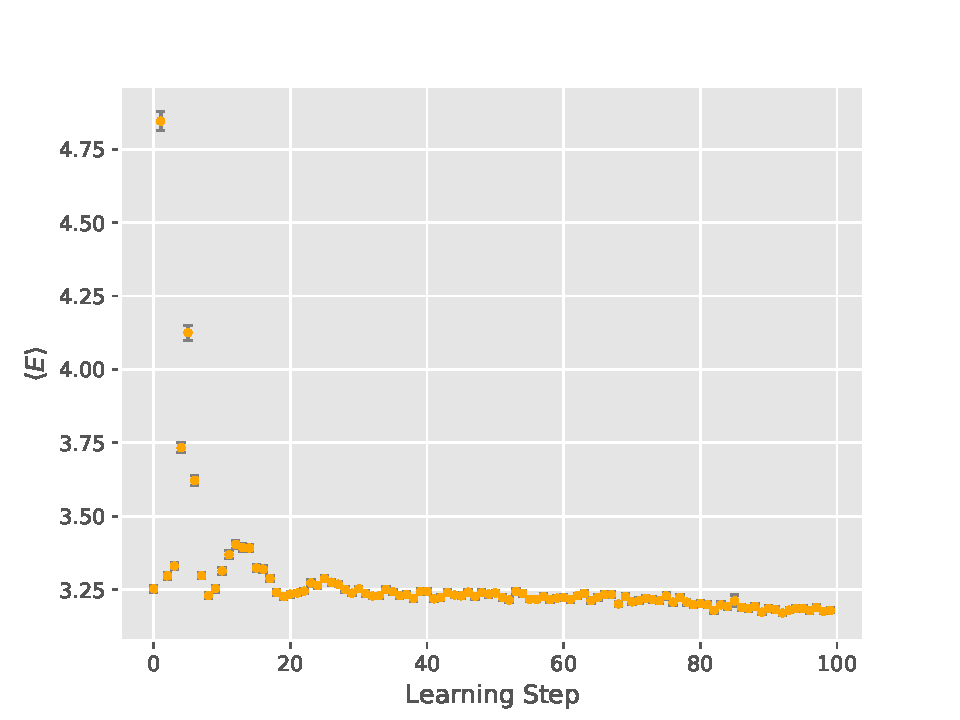
\includegraphics[trim=0cm 0.0cm 0cm 0cm,scale = 0.5]{D2_P_2I_Y__S_2pow20_eqS_2pow20_GD_ls_v_E_LR_0.200000_NH_6_Adaptive_1_Importance.pdf}
\caption{Importance sampling}
\label{J1}
\end{subfigure}
\begin{subfigure}[t]{.5\textwidth}
\centering
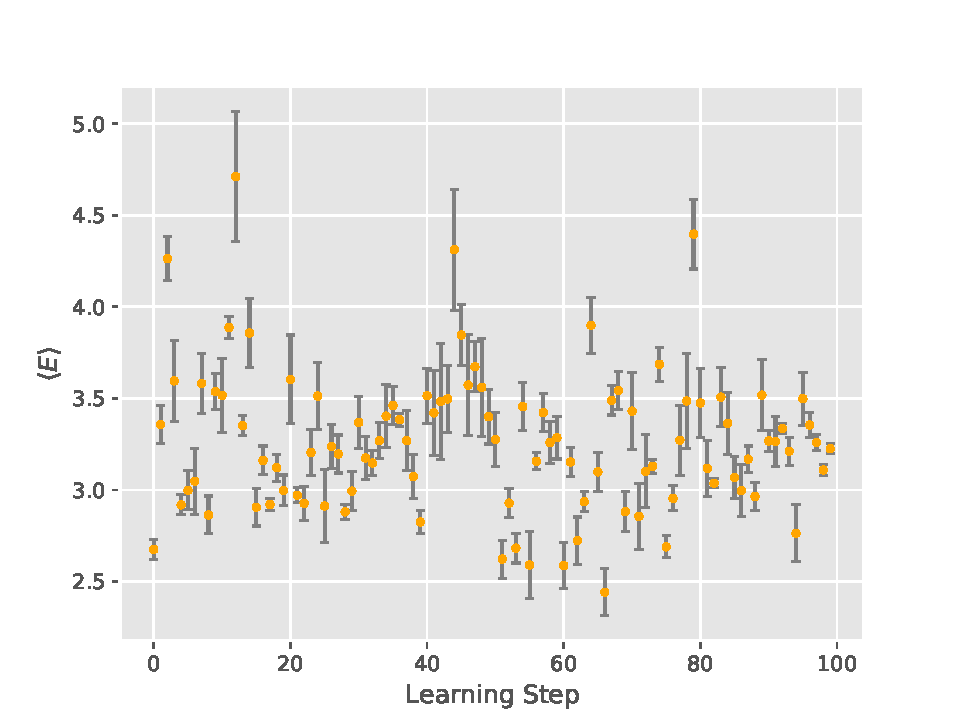
\includegraphics[trim=0cm 0.0cm 0cm 0.0cm,scale = 0.5]{D2_P_2I_Y__S_2pow20_eqS_2pow20_GD_ls_v_E_LR_0.200000_NH_6_Adaptive_1BruteForce.pdf}
\caption{Brute force}
\label{J2}
\end{subfigure}
\caption[Brute force v. Importance sampling]{Two Interacting electrons in two dimensions with 6 hidden nodes. Computed using $2^{20}$ equilibration steps, $2^{20}$ sampling steps. Expectation values for the local energy (a.u.) as a function of learning step upto 100 ADAM learning steps with a learning rate of $0.2$. The expectation values and standard deviations were calculated using blocking.}
\label{fig:BF_v_importance}
\end{figure}
We see that brute force sampling gives much higher errors and a much lower rate of convergence, including giving much lower estimates than the theoretical minimum of $3a.u.$ for some runs. This is indicative of the system undergoing too few Monte- Carlo cycles. Because of this, all remaining results are calculated using importance sampling.


\subsubsection{Adam v. SGD}
In figures \ref{fig:ADAM_v_SGD} and \ref{fig:ADAM_v_SGD2} we compare the two different implemented methods for optimizing the network parameters. First with a learning rate of $0.01$ then $0.1$. 

\begin{figure}[H]
\begin{subfigure}[t]{.5\textwidth}
\centering
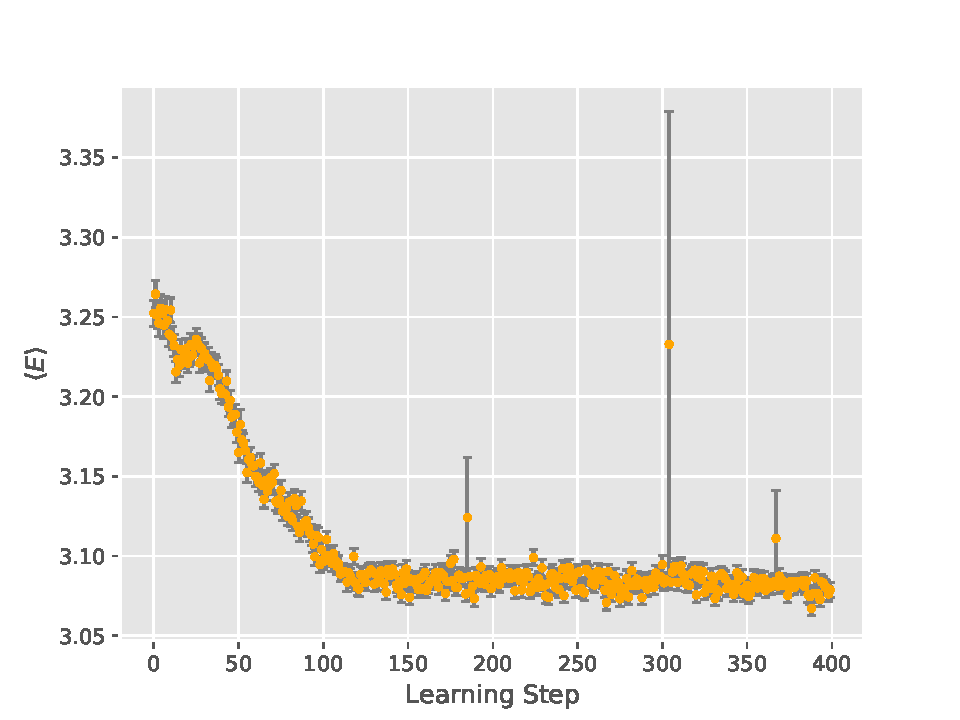
\includegraphics[trim=0cm 0.0cm 0cm 0cm,scale = 0.5]{D2_P_2I_Y__S_2pow21_eqS_2pow21_GD_ls_v_E_LR_0.010000_NH_3_Adaptive_1.pdf}
\caption{ADAM}
\label{ADAM}
\end{subfigure}
\begin{subfigure}[t]{.5\textwidth}
\centering
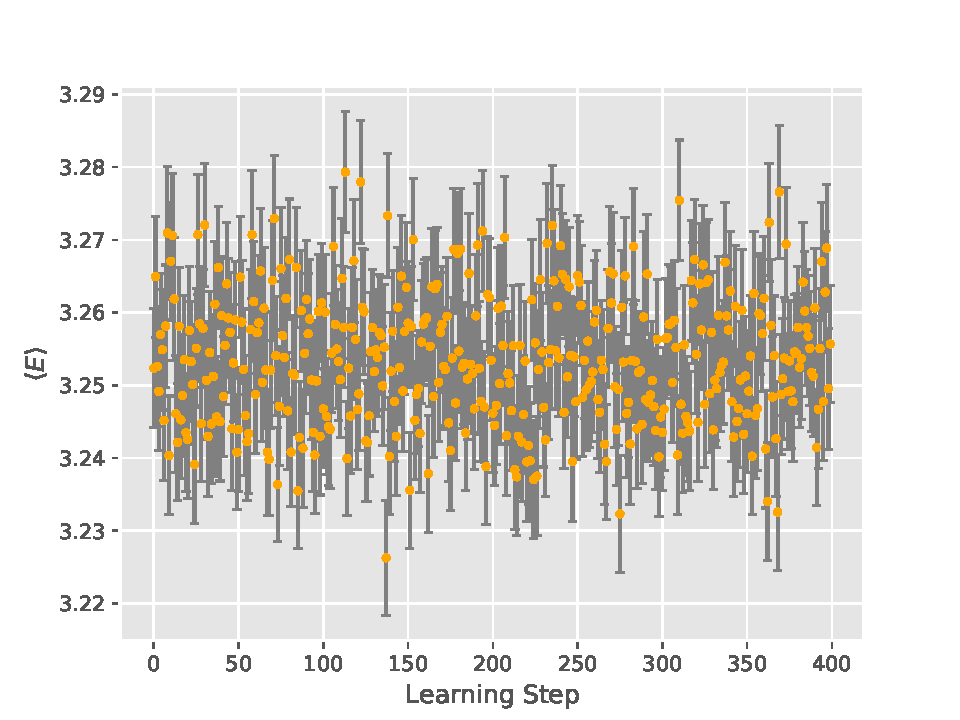
\includegraphics[trim=0cm 0.0cm 0cm 0.0cm,scale = 0.5]{D2_P_2I_Y__S_2pow21_eqS_2pow21_GD_ls_v_E_LR_0.010000_NH_3_Adaptive_0.pdf}
\caption{SGD}
\label{SGD}
\end{subfigure}
\caption[SGD v. ADAM]{2 interacting particles in 2 dimensions. Expectation values for the local energy (a.u.) as a function of learning step using a learning rate of $0.01$. 3 hidden nodes, $2^{21}$ metropolis- Hastings steps and $2^{21}$ equilibration steps. }
\label{fig:ADAM_v_SGD}
\end{figure}

\begin{figure}[H]
\begin{subfigure}[t]{.5\textwidth}
\centering
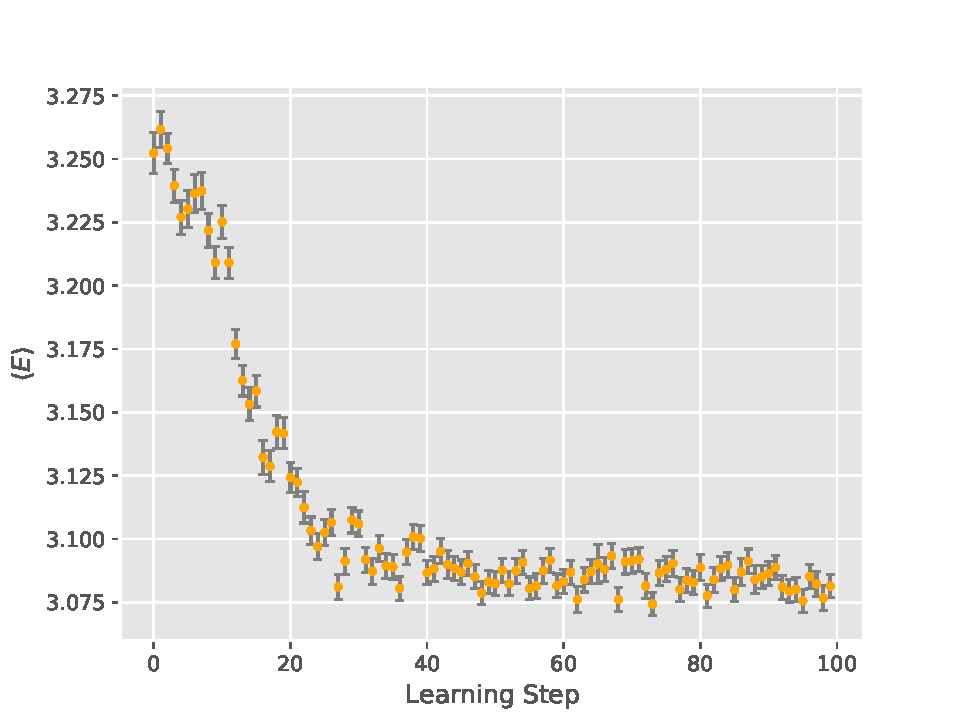
\includegraphics[trim=0cm 0.0cm 0cm 0.0cm,scale = 0.5]{D2_P_2I_Y__S_2pow21_eqS_2pow21_GD_ls_v_E_LR_0.100000_NH_3_Adaptive_1.pdf}
\caption{ADAM}
\label{ADAM2}
\end{subfigure}
\begin{subfigure}[t]{.5\textwidth}
\centering
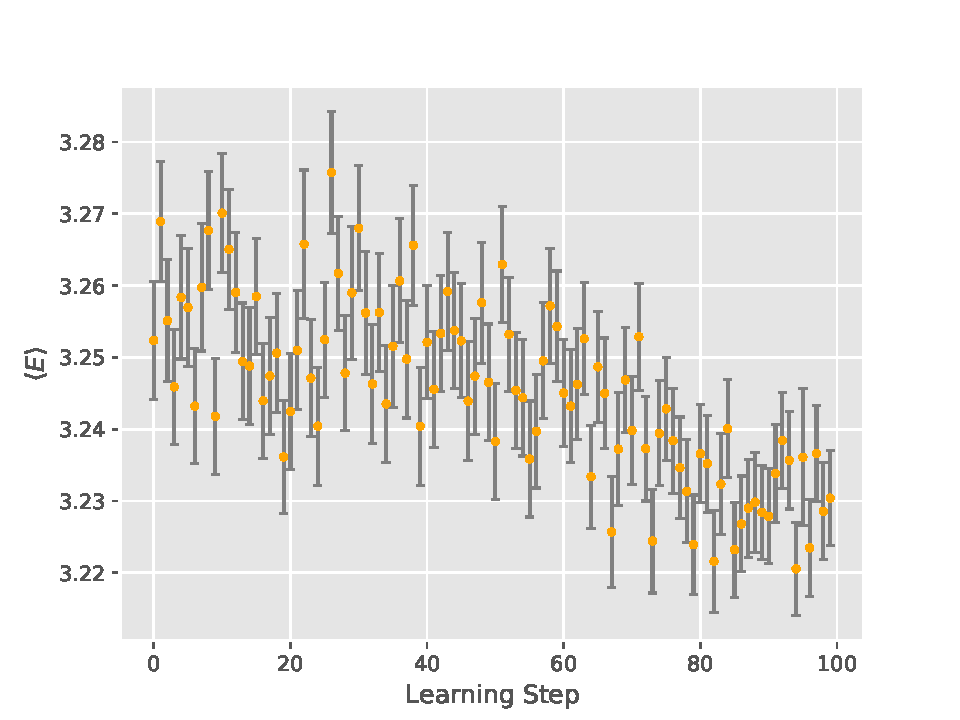
\includegraphics[trim=0cm 0.0cm 0cm 0.0cm,scale = 0.5]{D2_P_2I_Y__S_2pow21_eqS_2pow21_GD_ls_v_E_LR_0.100000_NH_3_Adaptive_0.pdf}
\caption{SGD}
\label{SGD2}
\end{subfigure}
\caption[SGD v. ADAM high learning rate]{2 interacting particles in 2 dimensions. Expectation values for the local energy (a.u.) as a function of learning step using a learning rate of $0.1$. 3 hidden nodes, $2^{21}$ metropolis- Hastings steps and $2^{21}$ equilibration steps. }
\label{fig:ADAM_v_SGD2}
\end{figure}

This isn't an entirely fair comparison since the learning rate plays a much more subtle role with ADAM compared to SGD. It does however highlight the central issue with fixed learning rate schemes. You want a large learning rate for fast convergence, and a small learning rate when you're close to the minimum. Both figures illustrates the point, which is to say that ADAM converges much more rapidly for both learning rates.\\ There are notable occurrences in figure \ref{ADAM}, namely three runs that had much higher energies and standard deviations compared to surrounding values. The surrounding values are still within one standard deviation of those results and so might be a statistical fluke, but they still stand out as perhaps being warning signs of unaccounted sources of systematic error.

\subsection{Non- interacting electrons}
The first set of numerical experiments relate to ground state energies for the trivial systems of one or two non- interacting electrons, whose analytic expressions are detailed in section \ref{section: Analytic_energies}. Figure \ref{fig:non_interacting_sweep} shows the calculated ground state energies of two non- interacting electrons for different ADAM learning rates and number of hidden nodes. This is only meant to be illustrative of the general trend, and instructive towards more in depth runs.
\begin{figure}[H]

\begin{subfigure}{.5\textwidth}
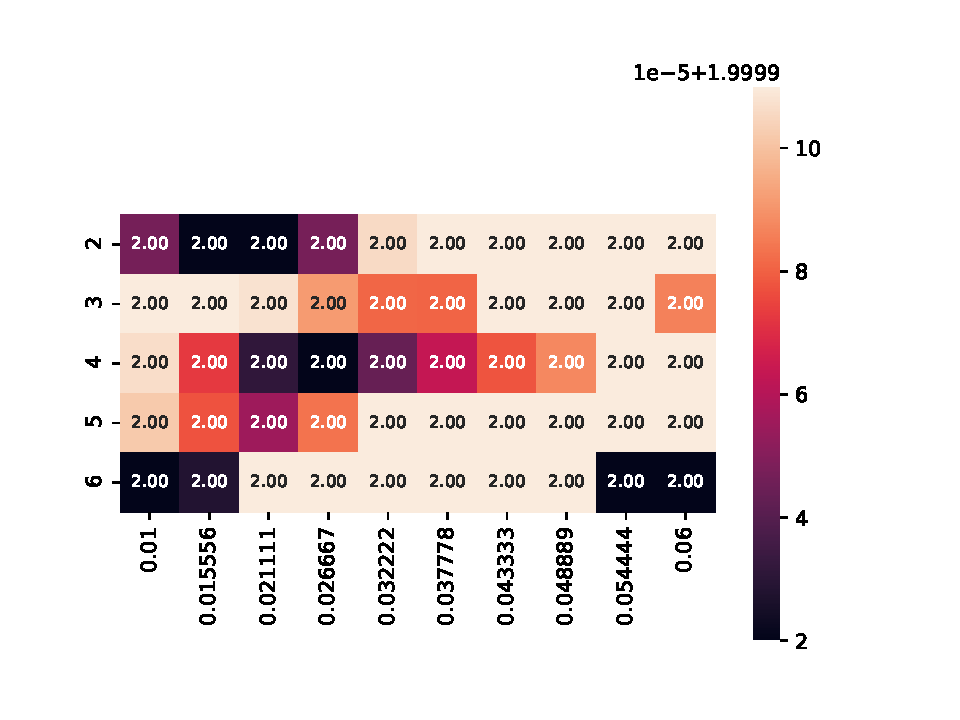
\includegraphics[trim=2cm 0.9cm 2cm 0.9cm,scale = 0.6]{exp_val.pdf}
\caption{Expectation value (a.u.)}\label{J1}
\end{subfigure}%
\begin{subfigure}{.5\textwidth}
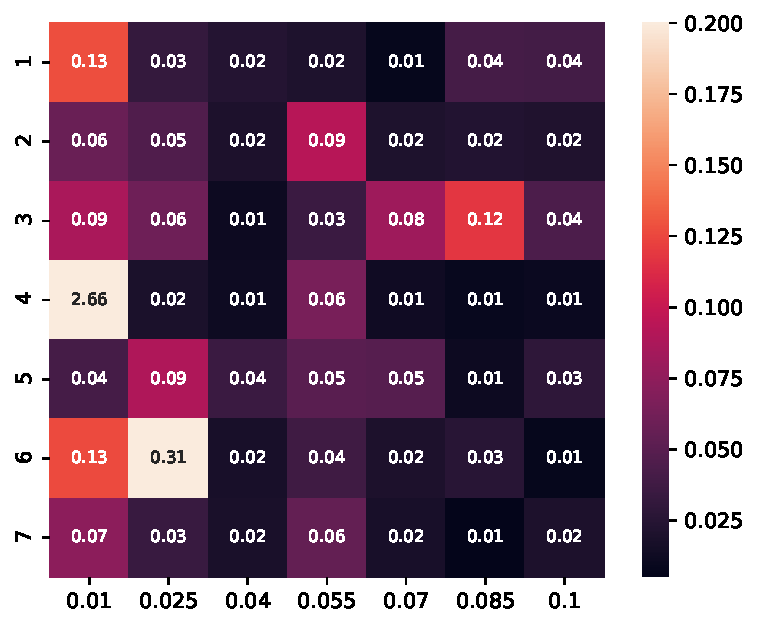
\includegraphics[trim=0cm 0.3cm 0cm 0.0cm,scale = 0.6]{std_dev.pdf}
\caption{standard deviation (a.u.)}\label{J2}
\end{subfigure}
\caption[Parameter sweep for two non- interacting electrons]{Two non- interacting electrons in two dimensions. Computed using importance sampling with $2^{20}$ equilibration steps, $2^{20}$ sampling steps and 50 ADAM learning steps. The number of hidden nodes on the y- axis and the learning rate on the x- axis. Expectation values and standard deviations were computed using blocking on the energies from the final learning step.}
\label{fig:non_interacting_sweep}
\end{figure}
The energies don't provide any unambiguous patterns except that lower learning rates seem to perform somewhat better. We see this again in the standard deviations, which have a clear trend towards lower learning rates. Initially the sectors with energies lower than $2a.u.$ are somewhat worrisome, but this seems to be accounted for, with standard deviations being somewhat higher for sectors with dark blue hues, and all standard deviations being above the threshold for bringing energies above $2a.u.$. It may of course also be the case that the energies are lower than $2(a.u.)$ due to some systematic error.\\\\ Without extensive searching, the energies for the trivial cases are provided in table \ref{table1} below.
\begin{table}[H]
\caption[Reproducing analytical results for trivial cases]{Expectation value for the local energy and standard deviation for the trivial systems. Using 20 ADAM learning steps with a learning rate of $0.01$, $2^{20}$ equilibration and sampling steps with importance sampling.}
\centering
\begin{tabular}{|l|l|l|l|l|}
\hline
Nr. Electrons & Nr. dimensions & $\hat{E}(a.u.)$          & $\sigma (a.u.) \times 10^{5}$ & Analytic $a.u.$\\ \hline
1             & 1              & 0.49999599 & 0.311658852                  & 0.5\\ \hline
1             & 2              & 0.99999918 & 0.568598342                  & 1.0\\ \hline
2             & 1              & 0.97796656 & 0.489544015                  & 1.0\\ \hline
2             & 2              & 2.00002012  & 1.060556                  & 2.0\\ \hline
\end{tabular}
\label{table1}
\end{table}

The 1- electron systems are in agreement with the analytic results to within one standard deviation. So is the 2- electron system in 2 dimensions. Worryingly, the 2- electron system in 1 dimension has a substantial discrepancy with the analytic result. 


\subsection{Interacting electrons}
For the interacting case, we again make a sweep of learning rates and number of hidden nodes, the result is shown in figure \ref{fig:interacting_sweep}.
\begin{figure}[H]
\begin{subfigure}{.5\textwidth}
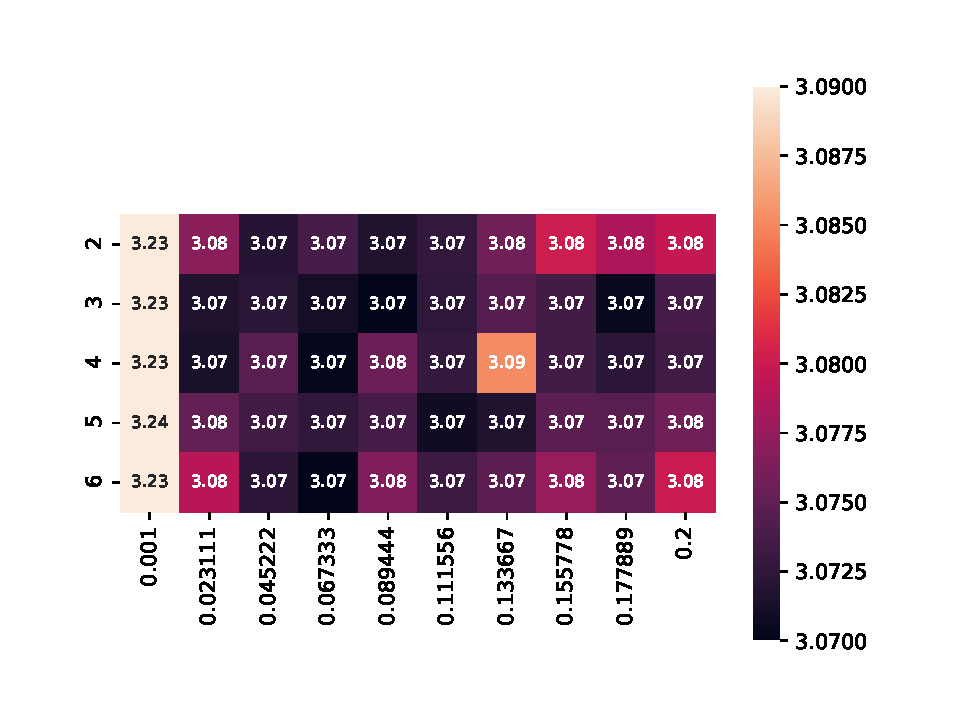
\includegraphics[trim=2cm 0.9cm 2cm 0.9cm,scale = 0.6]{exp_valInteracting.pdf}
\caption{Expectation value (a.u.)}\label{expectInteract}
\end{subfigure}%
\begin{subfigure}{.5\textwidth}
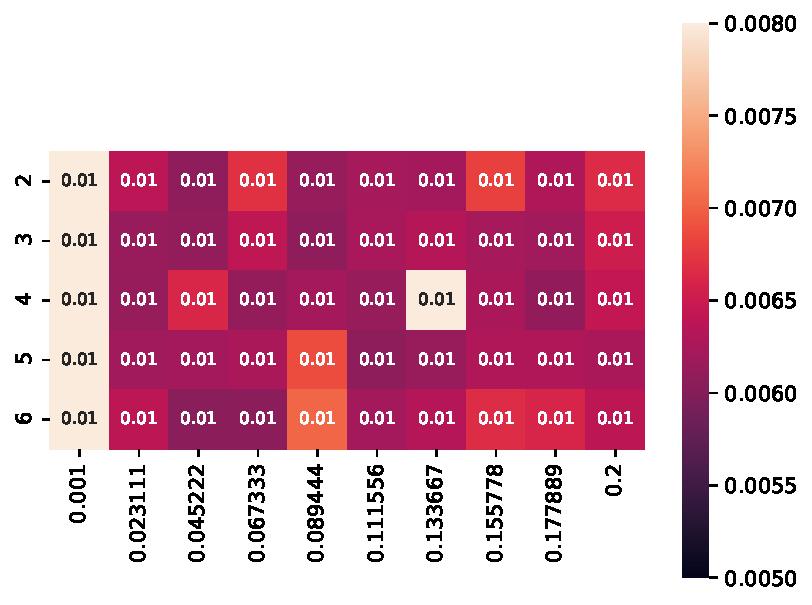
\includegraphics[trim=0cm 0.3cm 0cm 0.0cm,scale = 0.6]{std_devInteracting.pdf}
\caption{standard deviation (a.u.)}\label{J2}
\end{subfigure}
\caption[Parameter sweep for two interacting electrons]{Two interacting electrons in two dimensions. Computed using importance sampling with $2^{20}$ equilibration steps, $2^{20}$ sampling steps and 200 ADAM learning steps. The number of hidden nodes on the y- axis and the ADAM- learning rate on the x- axis. Expectation values and standard deviations were computed using blocking on the energies from the final learning step.}
\label{fig:interacting_sweep}
\end{figure}
We see from figure \ref{expectInteract} that a learning rate of $0.001$ initially, is not sufficient for the program to converge in the course of $200$ ADAM steps. Using this parameter sweep as a starting point and using the network parameters acquired at the final learning step for the learning rate $0.067$ and hidden node number $4$, successive runs with incrementally  smaller learning rates yielded the current best estimate of $3.04450717a.u.$ with a standard deviation of $0.01146434a.u.$ using a final learning rate of $0.00001$. Smaller learning rates and more computations could of course be attempted.

\subsection{Electron Locations}
Another measure of interest is how the electrons are distributed in space, and how that distribution changes from system to system. In figure \ref{fig:radial_oneAndTwo} we see the radial distribution of electrons from the center of the HO potential.
\begin{figure}[H]
\center
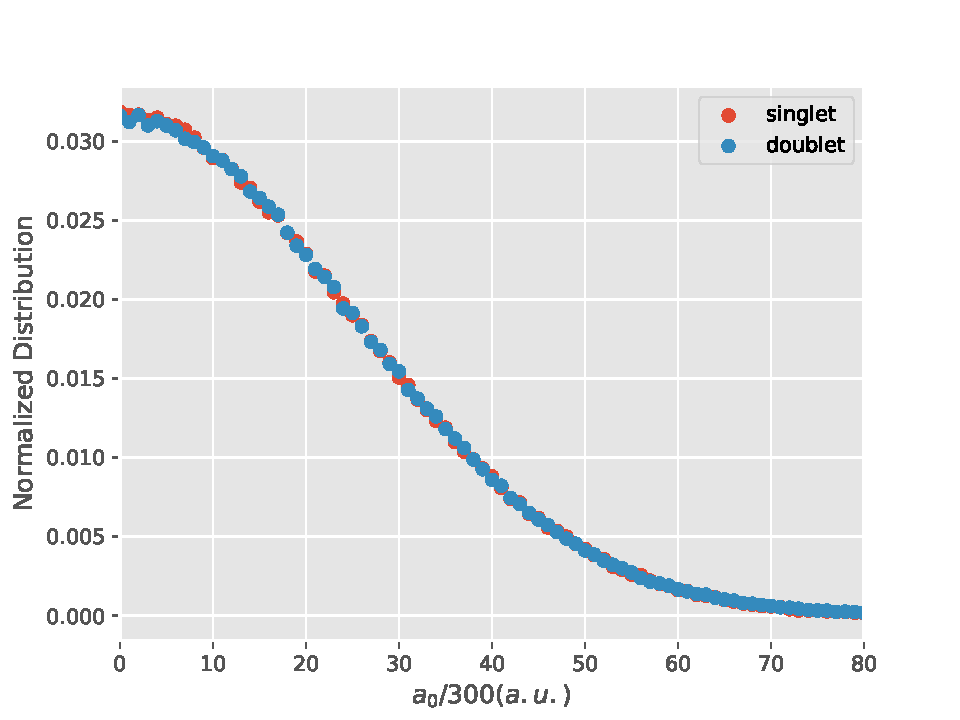
\includegraphics[trim=0cm 0.3cm 0cm 0.0cm,scale = 0.6]{Radial_distribution_One_v_Two.pdf}
\caption[Normalized radial distribution of singlet and non- interacting doublet]{Normalized radial distribution for the singlet and non- interacting doublet states in 1/600 of a Bohr radius, the natural length scale of the system. The energies are $1.0000 a.u.$ and $1.99997 a.u.$ for the singlet and doublet respectively. }
\label{fig:radial_oneAndTwo}
\end{figure}
Because the energy of two electrons is exactly twice that of one electron, and because the Hamiltonian doesn't couple to spin, this is exactly the result we expect to see. The normalized radial distribution for the singlet and doublet states are the same barring a very slight discrepancy toward the peak of the distribution, with very slightly fewer electrons inhabiting the near center of the potential.\\\\The spatial distributions of all 2- dimensional systems can be seen in figure \ref{fig:IMportance_pos_sampling}.

\begin{figure}[H]
\begin{subfigure}[t]{.5\textwidth}
\centering
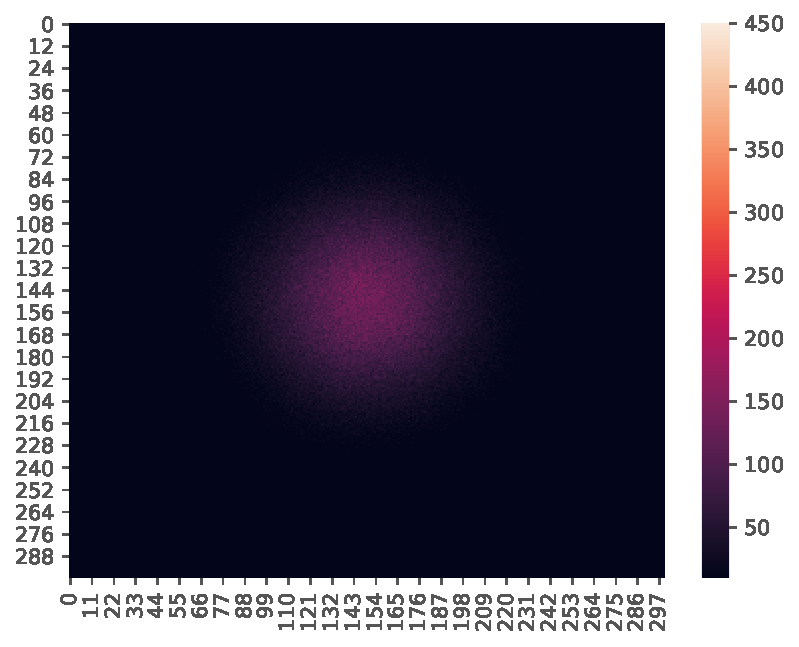
\includegraphics[trim=0cm 0.0cm 0cm 0cm,scale = 0.6]{D2_P_1I_N_Importance_S_2pow20_eqS_2pow20_Position_SamplingSingle_E1.pdf}
\caption{1 electron, $\hat E = 1$(a.u.)}
\label{imp1}
\end{subfigure}
\begin{subfigure}[t]{.5\textwidth}
\centering
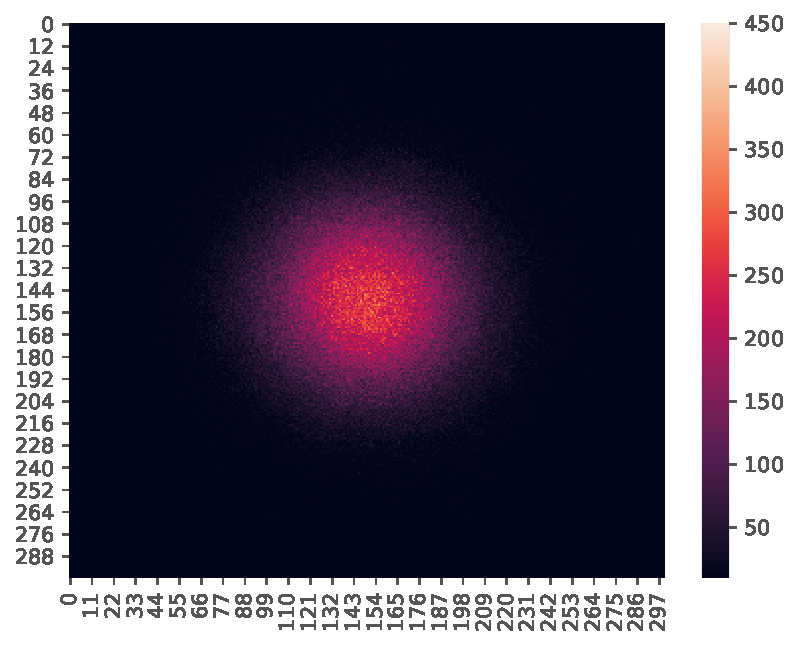
\includegraphics[trim=0cm 0.0cm 0cm 0.0cm,scale = 0.6]{D2_P_2I_N_Importance_S_2pow20_eqS_2pow20_Position_SamplingNON_interactingE1_9997.pdf}
\caption{2 electrons, $\hat E = 1.99997$(a.u.)}
\label{imp2}
\end{subfigure}
\begin{subfigure}[b]{.5\textwidth}
\centering
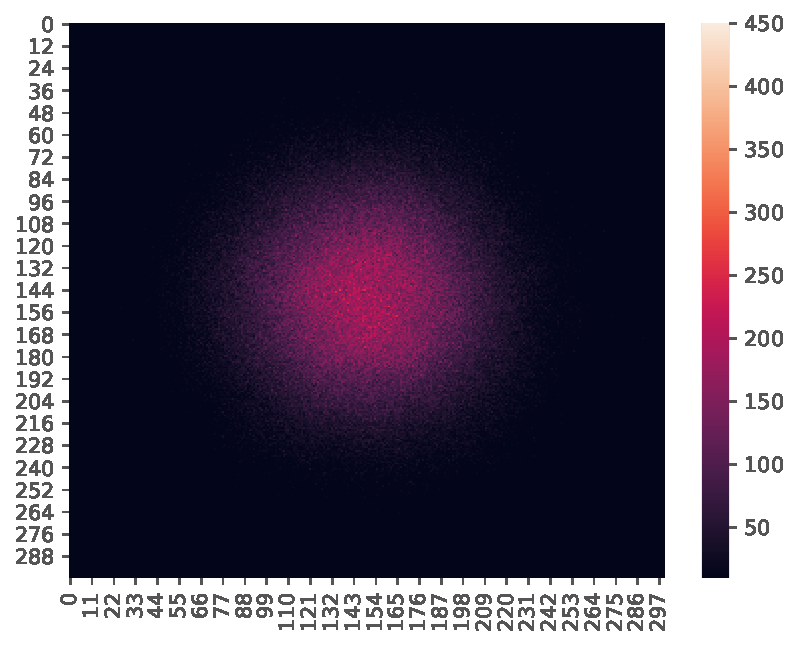
\includegraphics[trim=0cm 0.0cm 0cm 0.0cm,scale = 0.6]{D2_P_2I_Y_Importance_S_2pow20_eqS_2pow20_Position_Sampling_InteractingE3_07}
\caption{2 interacting electrons, $\hat E = 3.07$(a.u.)}
\label{imp3}
\end{subfigure}
\begin{subfigure}[b]{.5\textwidth}
\centering
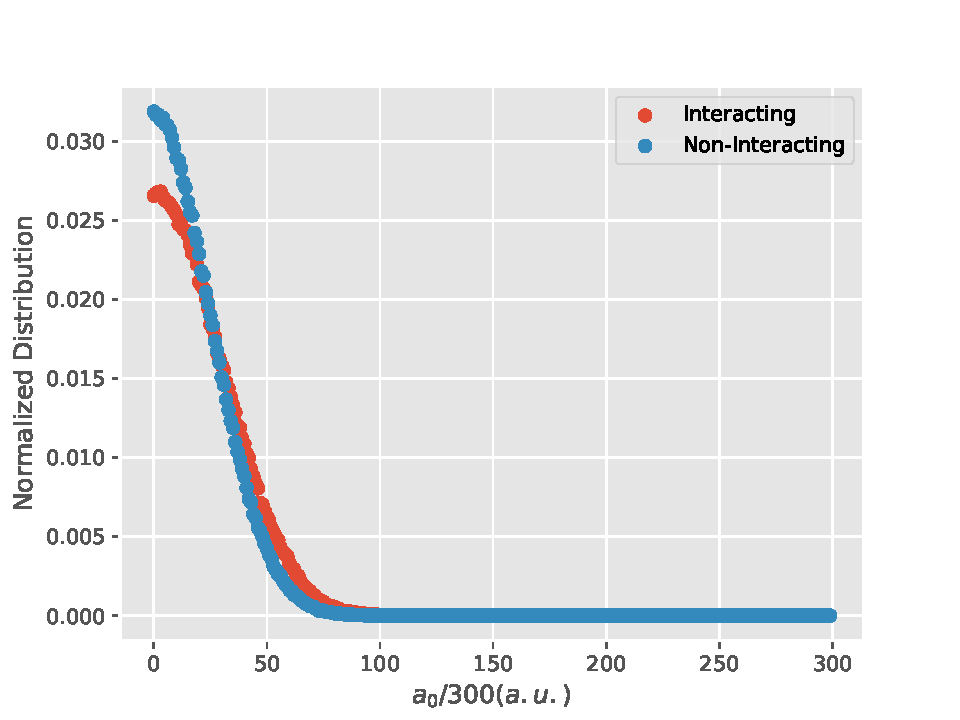
\includegraphics[trim=0cm 0.0cm 0cm 0.0cm,scale = 0.5]{Radial_distribution_interacting_v_Non.pdf}
\caption{Radial Distribution of 2 electrons with and without interaction $a_0 =  Bohr\hspace{1mm}radius/2$.}
\label{imp4}
\end{subfigure}
\caption[Spatial distribution of electrons]{Electrons in two dimensions. Computed using importance sampling with $2^{20}$ equilibration steps and $2^{20}$ sampling steps. The entire interval in the x and y positions are six times the natural length scale of the system, centered at $x,y =0$. Those intervals are split into 300 zones that record each time an electron is located in that zone in the course of the sampling steps. Note that the x- and y- axes in figures \ref{imp1}, \ref{imp2} and \ref{imp3} are given in 1/300th's of the Bohr radius, not $a_0$ as I've annoyingly managed to call half the Bohr radius in the radial distribution diagrams.}
\label{fig:IMportance_pos_sampling}
\end{figure}
Here we see exactly what we would expect. When the interaction is included, the electrons distribute themselves farther from the center of the HO potential to reduce the interaction potential. We see this both in the spatial distribution plot where the bright central spot is notably missing with the interaction, and in the radial distribution plot where electrons are shifting to between 40 and 80 $\frac{1}{600}th's$ of a Bohr radius from the center.

 
\section{Discussion}
\subsection{Loss of significance}
In the computation of equation \eqref{eq:doubleDerivativeFinal}, the term $(1-\zeta(u_j))$ will inevitably lead to loss of precision as $\zeta(u_j)$ takes on values $\{f \hspace{2mm}|\hspace{2mm} 0<f<1 \}$ and can therefore come very close to one. A solution would be to compute $\zeta(-u_j)$ instead.\\Loss of significance can happen many places in this program, but the unique shape of the Sigmoid makes it much more likely in this case.
\subsection{Divide by zero}
The interaction term of the Hamiltonian involves dividing by the absolute value of the distance between particles which may at some point during the simulation become zero. The implementation accounts for this by adding an epsilon of order $10^{-10}$ to denominator, which since we're taking the absolute value, should prevent any division by zero. This is not ideal, as it artificially lowers the computed energy. This method could potentially be improved by branching if the particle distance would lead to overflow, replacing the output with a value sufficiently below the overflow threshold.
\subsection{The nature of an upper bound}
Ideally, we would want for our program to come as absolutely close to the analytic value, from above, and never below it. Because of the inevitable shortcomings of floating point arithmetic, we would want to extensively catalogue the systematic sources of error and bias them if possible to over estimate (rather than under estimate) the energy of the system. This would be one of many necessary steps to making this program predictive in problems, not blessed by analytic solutions.
\subsection{Bug}
A bug in an earlier implementation of this program would sometimes cause the energy of the system to explode. Now, I wouldn't normally include details about a bug, except that this one was quite interesting. Because of an indexing error, the y- coordinate of the second particle would never be updated in a metropolis step. The same indexing error also meant that if the move was rejected, the program would do something like this

\begin{algorithm}[H]
\SetAlgoLined
set $P_1(y) = P_2(x)$\;
set $P_2(x) = P_2(y) = Constant$\;
\end{algorithm}
effectively constraining the second particle to move along a small vertical line.
This meant that every time two moves were rejected in a row, we would get

\begin{algorithm}[H]
\SetAlgoLined
\KwResult{$P_1(y) = P_2(x) = P_2(y) = Constant$}
set $P_1(y) = P_2(x)$\;
set $P_2(x) = P_2(y)$\;
set $P_1(y) = P_2(x)$\;
set $P_2(x) = P_2(y)$\;
\end{algorithm}
This would (less strictly) constrain the first particle to align with the second, horizontally. The only (actual) degree of freedom for the system then became the x- position of the first particle. This created an obvious failure mode where every time the first particle crossed a diagonal ($P_1(x) = P_1(y)$), the interaction term would explode. The chance then, that the only relevant parameter ($P_1(x)$) would be updated in the next cycle was less than 1 in 3. The energy would then aggregate over several cycles and likely cause a memory leak. This problem would become worse, the closer the initial value of $P_2(y)$ was to zero, as the first particle would intercept the diagonal more frequently near the origin.\\One example of this failure mode is seen in figure \ref{fig:posSampling_unstable} below. The diagonal is marked in red. The x- and y- axes are flipped.
\begin{figure}[H]
\center
\begin{tikzpicture}
\node[inner sep=0pt] (russell) at (0,0)
    {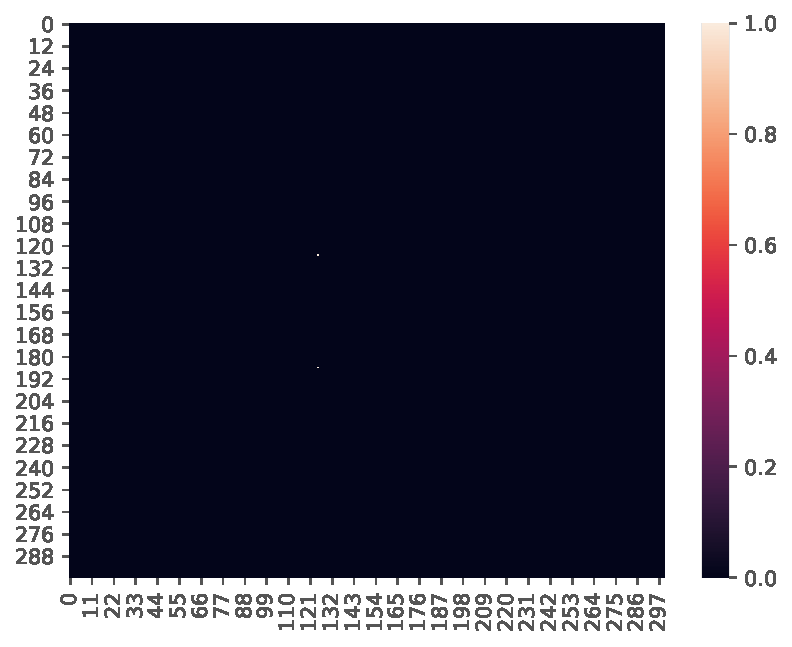
\includegraphics[trim=0cm 0.3cm 0cm 0.0cm,scale = 0.6]{D2_P_2I_Y_Importance_S_2pow19_eqS_2pow18_Position_sampling_P_2_NH_2_I_1_Ene_ne1374.pdf}
};
\draw[red, thick, opacity = 0.1] (-3.4,3.0) -- (2.8,-2.7);
\end{tikzpicture}
\caption[numerically unstable run- electron positions]{Position sampling for 2 interacting electrons in 2 dimensions using importance sampling. In this case, the energy was calculated to be $-1374\hspace{1mm} a.u.$ The electrons remained at those locations for every sampling step. The second particle (most likely) is located on a diagonal, and the first (most likely) is horizontally locked to it.}
\label{fig:posSampling_unstable}
\end{figure}



\section{Conclusion}
The application of RBMs to systems of interacting electrons has been shown to be worthwhile, and largely successful. Using good optimization schemes and reducing statistical errors have been the most fruitful endeavours in getting good estimates. The optimization can only work well as long as the random fluctuations in expectation values between optimization runs don't exceed the incremental improvements made by tweaking the parameters. For this, importance sampling and the ADAM optimizer proved to be best options. The number of hidden nodes in the wave function made close to no difference in its predictions. Using very small ADAM learning rates (0.00001) close to the minimum for the energy was very effective in further minimizing the energy.\\\\The program seems to be largely in agreement with analytical results except for two electrons in one dimension, where it underestimated the energy by over $0.023 a.u.$. This is a very big disparity that seriously undermines the predictive power of the program. Either more Monte- Carlo cycles are needed or there are systematic sources of error that would need to be addressed.\\The program gave a quite accurate upper bound for the interacting system with $3.04450717a.u.$ compared to $3.0a.u.$ for the analytic solution with a standard deviation of $0.01146434a.u.$\\\\This implementation is not currently in a good state for making predictions. It should be in much greater agreement with theory and provide thorough details about the sources of error in this program. It would therefore benefit greatly from a host of unit tests to pinpoint the main contributors.\\\\To expand the breadth of this program one would need to implement new waveFunction and Hamiltonian daughter classes to incorporate the Pauli exclusion principle, spin coupling and potentially external magnetic fields. This would in turn require a method of numerical differentiation of the wave function, unless analytic derivatives for such wave functions exist.

\section{Appendix A}\label{app_A}
Using the hamiltonian in \eqref{eq:hamiltonian} we get that the local energy is given by
$$
\begin{aligned}
E_{L} &=\frac{1}{\Psi} \mathbf{H} \Psi \\
&=-\frac{1}{2} \frac{1}{\Psi} \sum_{i}^{M} \frac{\partial^2}{\partial X_i^2} \Psi+\frac{1}{2} \omega^{2} \sum_{i}^{M} X_{i}^{2}+\sum_{j<k} \frac{1}{r_{j k}}
\end{aligned}
$$
with $M$ being the number of visible nodes in the network. The only non- trivial contribution comes from the Laplacian. We can simplify the differential term like this
$$
\frac{\partial^2}{\partial X_i^2} ln\Psi = \frac{\partial}{\partial X_i}\left( \frac{1}{\Psi}\frac{\partial}{\partial X_i} \Psi \right) = \frac{1}{\Psi}\frac{\partial^2}{\partial X_i^2} \Psi - \left( \frac{\partial}{\partial X_i} ln\Psi \right)^2
$$
giving us this expression

\begin{equation}\label{eq:local_energy_derived}
\begin{aligned}
E_{L} &=\frac{1}{\Psi} \mathbf{H} \Psi \\
&=-\frac{1}{2} \sum_{i}^{M} \left( \frac{\partial^2}{\partial X_i^2} ln\Psi +  \left( \frac{\partial}{\partial X_i} ln\Psi \right)^2 \right)+\frac{1}{2} \omega^{2} \sum_{i}^{M} X_{i}^{2}+\sum_{j<k} \frac{1}{r_{j k}}.
\end{aligned}
\end{equation}
The natural log of the wave function is computed to be
$$
ln\Psi = -ln Z-\sum_{i}^{M} \frac{\left(X_{i}-a_{i}\right)^{2}}{2 \sigma^{2}}+\sum_{j}^{N} ln \left(1+e^{b_{j}+\sum_{i}^{M} \frac{X_{i} W_{i j}}{\sigma^{2}}}\right).
$$
The differentials can then be solved to get
$$
\frac{\partial}{\partial X_i} ln \Psi=\frac{1}{\sigma^{2}}\left(a_i-X_i+\sum_{j}^{N} W_{ij}\zeta(u_j) \right)
$$
and
$$
\frac{\partial^{2}}{\partial X_{i}^{2}} ln \Psi=-\frac{1}{\sigma^{2}}+\frac{1}{\sigma^{4}} \sum_{j}^{N} W_{i j}^{2} \zeta(u_j) \zeta(-u_j) 
$$
\begin{equation}\label{eq:doubleDerivativeFinal}
\frac{\partial^{2}}{\partial X_{i}^{2}} ln \Psi=-\frac{1}{\sigma^{2}}+\frac{1}{\sigma^{4}} \sum_{j}^{N} W_{i j}^{2} \zeta(u_j) (1-\zeta(u_j))
\end{equation}
where $\zeta_j = \frac{1}{e^{-u_j}+1}$ is the familiar sigmoid function with $u_j = b_{j}+\frac{1}{\sigma^{2}} \sum_{k}^{M} X_k W_{k j}$. This concludes the calculation.
\section{Appendix B}\label{app_B}
The gradient of the local energy with respect to the network parameters is given by
\begin{equation}\label{eq:lE_gradient}
G_{i}=\frac{\partial\left\langle E_{L}\right\rangle}{\partial \alpha_{i}}=2\left(\left\langle E_{L} \frac{1}{\Psi} \frac{\partial \Psi}{\partial \alpha_{i}}\right\rangle-\left\langle E_{L}\right\rangle\left\langle\frac{1}{\Psi} \frac{\partial \Psi}{\partial \alpha_{i}}\right\rangle\right).
\end{equation}
From the expression for the wave function in \ref{app_A} the derivative of the wave function with respect to the weights and biases are calculated to be
$$
\frac{\partial}{\partial a_{i}} ln \Psi =\frac{X_{i}-a_{i}}{\sigma^{2}},
$$
$$
\frac{\partial}{\partial b_{i}} ln \Psi = \zeta_i
$$
and
$$
\frac{\partial}{\partial W_{i j}} ln \Psi =\frac{X_{i}}{\sigma^{2}}\zeta_j.
$$
this concludes the calculation.
\bibliographystyle{plain}
\bibliography{references}
\end{document}
